\textbf{Ejemplo 3}\\
Una persona debe cancelar la suma de 2{.}000{.}000 COP al cabo de 18 meses. ¿Cuál debe ser el valor del ahorro que debe hacer hoy en una cuenta que paga el equivalente al 24\% nominal anual trimestre vencido (natv) para poder cancelar la deuda?\\

%%%%%%%%%%%%%%%%%%% EJERCICIO 1 %%%%%%

%\newpage %USAR SOLO SI EL SOLUCIÓN QUEDA SOLO Y ES NECESARIO BAJARLO A LA SIGUIENTE PAGINA
\textbf{Solución.}\\
%La tabla ira centrada
\begin{center}
  \renewcommand{\arraystretch}{1.5}% Margenes de las celdas
  %Creación de la cuadricula de 3 columnas \end{flushleft}
  \begin{longtable}[H]{|C{0.3\linewidth}|C{0.3\linewidth}|C{0.3\linewidth}|}
    %Creamos una linea horizontal
    \hline
    %Definimos el color de la primera fila
    \rowcolor[HTML]{FFB183}
    %%%%% INICIO ASIGNACIÓN FECHA FOCAL %%%%%%%
    %%%%%%%%%% INICIO TITULO
    %Lo que se hace aquí es mezclar las 3 columnas en una sola
    \multicolumn{3}{|c|}{\cellcolor[HTML]{FFB183}\textbf{1. Asignación período focal}}                                  \\ \hline
    %%%%%%%%%% FIN TITULO
    %%%%% INICIO DECLARACIÓN DE VARIABLES %%%%%%%
    \multicolumn{3}{|c|}{$pf = 0ptv$}                                                                                   \\ \hline
    %%%%%%%%%% INICIO TITULO
    %Lo que se hace aquí es mezclar las 3 columnas en una sola
    \multicolumn{3}{|c|}{\cellcolor[HTML]{FFB183}\textbf{2. Declaración de variables}}                                  \\ \hline
    %%%%%%%%%% FIN TITULO
    %%%%%%%%%% INICIO DE MATEMÁTICAS
    %Cada & hace referencia al paso de la siguiente columna
    $F =   2{.}000{.}000$ COP & $j=24\%natv$                     & $P= ?$ COP                                        \\
                               & $i=\frac{24\%natv}{4ptv}=6\%ptv$ &                                                     \\ & $n=\frac{18pmv}{3pmv}=6ptv$ &
    \\\hline

    %%%%%%%%%% FIN DE MATEMÁTICAS
    %%%%% FIN DECLARACIÓN DE VARIABLES


    %%%%% INICIO FLUJO DE CAJA
    \rowcolor[HTML]{FFB183}
    \multicolumn{3}{|c|}{\cellcolor[HTML]{FFB183}\textbf{3. Diagrama de flujo de caja}}                                 \\ \hline
    %Mezclamos 3 columnas y pondremos el dibujo
    %%%%%%%%%%%%% INSERCIÓN DE LA IMAGEN
    %Deberán descargar las imágenes respectivas del drive y pegarlas en la carpeta
    %n_capitulo/img/ejemplos/1/capitulo1ejemplo1.pdf  (el /1/ es el numero del ejemplo)
    \multicolumn{3}{|c|}{ 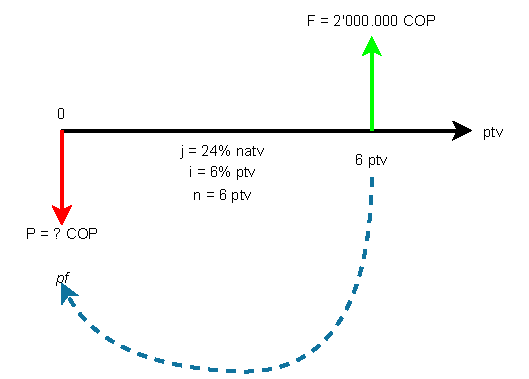
\includegraphics[trim=-5 -5 -5 -5 , scale=1]{2_Capitulo/ejemplos/3/Capitulo2Ejercicio3_v2.pdf} } \\ \hline
    %%%%%%%%%%%%% FIN INSERCIÓN DE IMAGEN
    %%%%%FIN FLUJO DE CAJA



    %%%%% INICIO DECLARACIÓN FORMULAS
    %%%%%%%%%%% INICIO TITULO
    \rowcolor[HTML]{FFB183}
    \multicolumn{3}{|c|}{\cellcolor[HTML]{FFB183}\textbf{4. Declaración de fórmulas}}                                   \\ \hline
    %%%%%%%%%%% FIN TITULO
    %%%%%%%%%%% INICIO MATEMÁTICAS
    \multicolumn{3}{|c|}{$F= P(1+i)^n\hspace{0.3cm} \textit{Valor futuro}$}                                             \\
    \multicolumn{3}{|c|}{$P= F(1+i)^{-n}\hspace{0.3cm} \textit{Valor presente}$}
    \\ \hline
    %%%%%%%%%% FIN MATEMÁTICAS
    %%%%%% INICIO DESARROLLO MATEMÁTICO
    \rowcolor[HTML]{FFB183}
    %%%%%%%%%%INICIO TITULO
    \multicolumn{3}{|c|}{\cellcolor[HTML]{FFB183}\textbf{5. Desarrollo matemático}}                                     \\ \hline
    %%%%%%%%%% FIN TITULO
    %%%%%%%%%% INICIO MATEMÁTICAS
    \multicolumn{3}{|c|}{$P=\frac{2{.}000{.}000 COP}{(1+0.06)^6}$}                                                   \\
    \multicolumn{3}{|c|}{$P=  1{.}409{.}920$ COP}
    \\ \hline


    %%%%%%%%%% FIN MATEMÁTICAS
    %%%%%% FIN DESARROLLO MATEMÁTICO
    %%%%%% INICIO RESPUESTA
    \rowcolor[HTML]{FFB183}
    %%%%%%%%%%INICIO TITULO
    \multicolumn{3}{|c|}{\cellcolor[HTML]{FFB183}\textbf{6. Respuesta}}                                                 \\ \hline
    %%%%%%%%%% FIN TITULO
    %%%%%%%%%% INICIO RESPUESTA MATEMÁTICA
    \multicolumn{3}{|c|}{$P= 1{.}409{.}920$ COP}                                                                   \\ \hline
    %%%%%%%%%% FIN MATEMÁTICAS
    %%%%%% FIN RESPUESTA
  \end{longtable}
  %Se crean dos lineas en blanco para que no quede el siguiente texto tan pegado
  %\newline \newline %USARLO SI CREES QUE ES NECESARIO
\end{center}
%%%%%%%%%%%%%%%%%%%%%%%%%%FIN EJERCICIO 1 %%%%%%%%%%%%%%%%%%%%%%%%%%%
